\RequirePackage[table]{xcolor}
\documentclass[fonts]{icst}

\usepackage{moreverb}

\usepackage[breaklinks,colorlinks,bookmarksopen,bookmarksnumbered,linkcolor=ICSTblue,citecolor=blue,urlcolor=ICSTblue]{hyperref}
\usepackage{breakurl}
\usepackage{doi}

\usepackage[utf8]{inputenc}
\usepackage[english]{babel}
\usepackage{amsmath,amssymb}
\usepackage{graphicx,flushend}
\usepackage{booktabs}
\usepackage{array}
\usepackage{multirow}
\usepackage{float}
\usepackage{enumitem}
\usepackage{dblfloatfix}
\usepackage{cuted}
\usepackage[hypcap=false]{caption}
\usepackage{adjustbox}
\usepackage{balance}
\newcommand\BibTeX{{\rmfamily B\kern-.05em \textsc{i\kern-.025em b}\kern-.08emT\kern-.1667em\lower.7ex\hbox{E}\kern-.125emX}}
\def\volumeyear{2024}
\journalname{XXXXXX}
\articletype{Research Article}
\setcounter{page}{01}
\def\volumeyear{XXXX}
\def\volumenumber{XX}
\def\issuemonth{XX-XX}
\def\issuenumber{X}
\def\articleid{XX}
\def\copyrightholder{Xuan-Huy Dinh\textit{ et al.}, licensed to ICST}
\copyrightnote{This is an open access article distributed under the terms of the Creative Commons Attribution license (\url{http://creativecommons.org/licenses/by/3.0/}), which permits unlimited use, distribution and reproduction in any medium so long as the original work is properly cited.}
\def\articledoi{10.4108/XX.X.X.XX}
\received{XXXX}
\accepted{XXXX}
\published{XXXX}

\begin{document}

\runningheads{}{}

\title{BiasLN: Efficient Tuning for Generalizable Deepfake Detection Across Benchmarks}

\author{Xuan-Huy Dinh,\ Minh-Duc Vu,\ Thanh-Quan Phung-Le,\ Duc-Thinh Nguyen,\ Van-Dung Hoang\fnoteref{1}}

\address{
    Faculty of Information Technology\\
    Ho Chi Minh City University of Technology and Engineering (HCMUTE)\\
    Ho Chi Minh City, Vietnam
}

\abstract{
Achieving robust generalization to unseen manipulation techniques remains a key challenge for existing detection models. Although Parameter-Efficient Fine-Tuning (PEFT) holds significant promise, existing approaches often rely on complex adaptation schemes that can disrupt pre-trained representations or lead to overfitting. To address this issue, we introduce BiasLN, a simple effective PEFT strategy that achieves good performance. Instead of incorporating additional modules that increase model complexity, we fine-tune only the bias terms and LayerNorm parameters of a pre-trained image encoder. This design preserves the core visual knowledge learned during pre-training while enhancing the model's ability to capture subtle manipulation artifacts that more complex architectures may overlook or overfit to. Experimental results demonstrate that BiasLN is resource-efficient and achieves competitive performance across multiple benchmarks. The proposed approach shows that a simple parameter-efficient design supports to improve generalization in deepfake detection.
}

\keywords{Deepfake detection, parameter-efficient fine-tuning,LayerNorm tuning}

\fnotetext[1]{Corresponding author. Email: \email{dunghv@hcmute.edu.vn}}

\maketitle

\section{Introduction}
The rapid growth of generative models, especially GANs~\cite{goodfellow2020gan} and diffusion models~\cite{yang2022diffusion}, has drawn significant attention in recent years. However, these advances also introduce serious risks, particularly their potential misuse for creating realistic fake face videos. Therefore, developing effective forgery detection models is essential.

Traditional detectors often rely on CNNs or frequency-domain artifacts. However, modern generative methods continue to minimize these local errors, making them increasingly difficult to detect using standard approaches.
This shift has led the field toward vision foundation models like CLIP and DINO~\cite{radford2021clip_vitl,caron2021emerging}.
These models offer robust, global representations that have already shown significant promise in "universal" detection tasks~\cite{ojha2023universal}.

However, fully fine-tuning these large models often leads to catastrophic forgetting, which reduces their generalization ability~\cite{kumar2022finetuning}.
To address this issue, Parameter-Efficient Fine-Tuning (PEFT) has emerged as a promising alternative. Recent methods such as Effort~\cite{yan2025effort} and GenD~\cite{yermakov2025gend} achieve strong cross-dataset performance by adapting models in different spaces, such as weight space or feature space.
Despite their effectiveness, these approaches introduce additional complexity, raising the question of whether such designs are truly necessary for robust deepfake detection.

We introduce BiasLN, a simple parameter-efficient fine-tuning strategy that updates only the bias terms and LayerNorm affine parameters of a pre-trained vision encoder while keeping all other weights frozen. This design provides sufficient adaptation capacity while preserving pre-trained knowledge.

We evaluate BiasLN under both cross-dataset and cross-method settings. Following the protocol of Effort~\cite{yan2025effort}, the model is trained on a single source dataset, selected using a held-out validation set, and evaluated on five unseen datasets as well as seven single-method benchmarks. Our results further highlight the importance of validation-set selection for robust generalization and show that BiasLN outperforms than recent state-of-the-art methods.

In summary, our key contributions are as follows:
\begin{enumerate}
    \item \textbf{A simple and effective method:} BiasLN updates only the bias and LayerNorm parameters of a vision encoder,  outperforms recent state-of-the-art methods in both cross-dataset and cross-method evaluations.

    \item \textbf{Extensive generalization evaluation:} Extensive experiments on five unseen datasets and seven single-method benchmarks demonstrate the robustness of BiasLN against diverse manipulations.

    \item \textbf{Robust model selection:} Prolonged training on a single dataset can still lead to overfitting, highlighting the importance of a strong validation set for selecting model weights that generalize reliably out of domain.
\end{enumerate}
At a high level, BiasLN starts from a frozen CLIP vision encoder and updates only its bias and LayerNorm parameters, while keeping all other weights fixed.
A lightweight classification head is trained on top of the adapted features for real/fake prediction.

The official source code is updated at \href{https://github.com/ducthinh4477/BiasLN}{GitHub}


\section{Related Work}

Generalizable deepfake detection remains difficult because many detectors overfit to dataset-specific artifacts. Early methods mainly relied on CNNs, frequency cues, or reconstruction signals to detect facial manipulations~\cite{rossler2019ff,luo2021srm,liu2021spsl,cao2022recce,badr2025wavit}. Although effective in-domain, these approaches often degrade on unseen forgeries because they depend heavily on low-level or method-specific artifacts.

To address this limitation, recent research has expanded from facial manipulation detection to broader AI-generated image detection and increasingly adopts vision foundation models, particularly CLIP, to improve cross-domain generalization~\cite{ojha2023universal,cui2025forada,yan2025effort,yermakov2025gend}. These methods can be grouped by their adaptation strategies. ForAda~\cite{cui2025forada} introduces a lightweight parallel adapter network to explicitly learn blending boundaries alongside the original vision-language model. Effort~\cite{yan2025effort} instead operates in parameter space through Singular Value Decomposition (SVD), freezing principal components and fine-tuning residual low-rank components to preserve pre-trained knowledge. Building on this parameter-efficient direction, GenD~\cite{yermakov2025gend} further reduces the trainable footprint by updating only LayerNorm parameters and complementing this design with feature-space objectives, including a uniform loss on the $L_2$ hypersphere and an alignment loss that pulls same-class samples closer together.

Compared with these more sophisticated approaches, BiasLN simply tunes only bias and LayerNorm parameters. This simple design provides sufficient capacity to learn deepfake manipulation traces while better preserving the pretrained representations, avoiding the need for additional architectural branches or multi-objective training losses.
 

\section{Methodology}
\label{sec:method}

We propose \textbf{BiasLN}, a simple parameter-efficient fine-tuning framework for generalizable deepfake detection. BiasLN freezes the pre-trained CLIP visual encoder and tunes only bias and LayerNorm affine parameters, preserving the pre-trained feature space while adapting the model to binary real/fake classification. Motivated by Effort~\cite{yan2025effort} and related PEFT methods such as BitFit~\cite{benzaken2022bitfit} and LayerNorm tuning~\cite{wang2022ln}, this design aims to improve cross-domain generalization with only a small number of trainable parameters.

\begin{figure}[H]
    \centering
    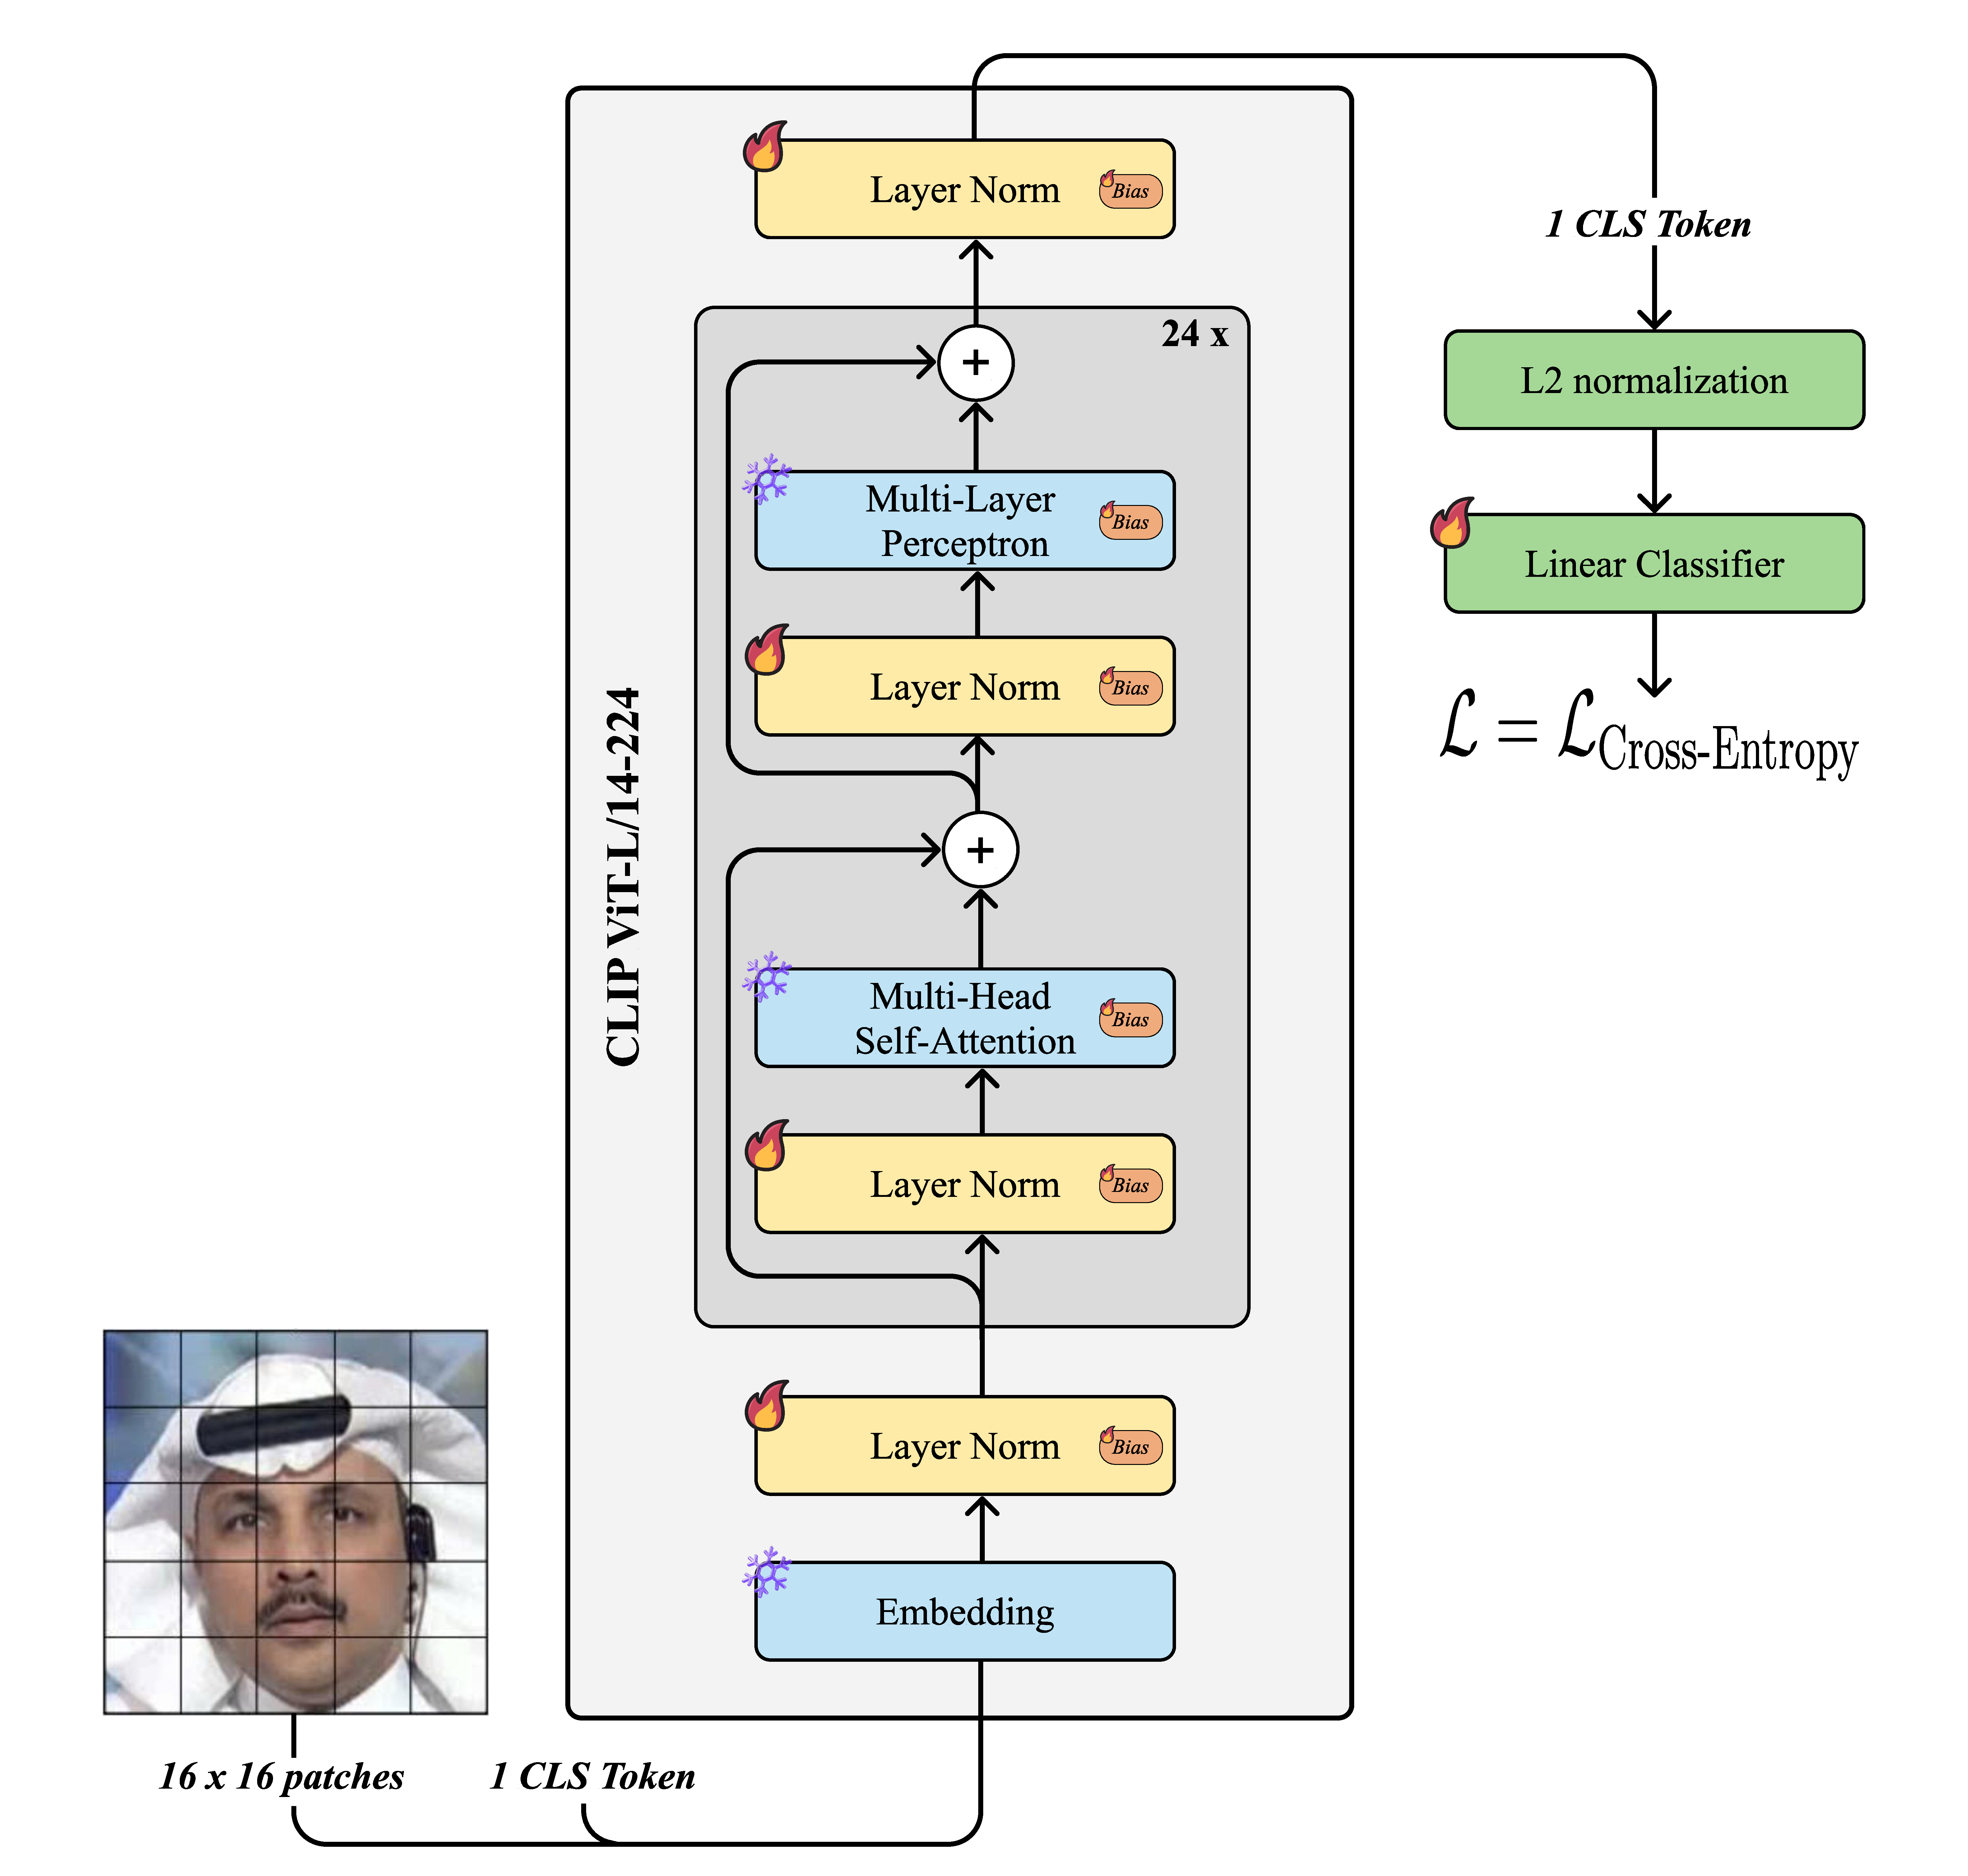
\includegraphics[width=\linewidth]{BiasLN.pdf}
    \caption{Overview of BiasLN.
The CLIP ViT-L/14 backbone is kept frozen except for bias terms and LayerNorm parameters, and the extracted features are passed to a lightweight classifier for deepfake detection.}
    \label{fig:model}
\end{figure}

\subsection{Feature Extractor}

Given an input image $\mathbf{x}$, the CLIP visual encoder~\cite{radford2021clip_vitl} extracts a global feature representation
\begin{equation}
\mathbf{f} = g_{\theta}(\mathbf{x}),
\end{equation}
where $\mathbf{f} \in \mathbb{R}^{1024}$ denotes the output of the CLS token.
To prevent catastrophic forgetting and rank collapse in the foundation model, the entire core parameter space of $g_{\theta}$---including projection matrices, attention weights, and feed-forward weights---remains frozen during training.
Adaptation to the deepfake detection task is therefore delegated to a highly constrained parameter-efficient fine-tuning strategy.

\subsection{Parameter-Efficient Fine-Tuning (PEFT) Strategy}
\label{sec:peft}

Rather than fine-tuning the full CLIP backbone, we adopt a minimal parameter update scheme that we term \textbf{BiasLN}.
This strategy combines two lightweight tuning mechanisms to preserve the structural integrity of the pre-trained model while still enabling effective adaptation to the target domain.

\paragraph{BitFit (Bias-only Tuning).}
Introduced by Ben Zaken et al.~\cite{benzaken2022bitfit}, BitFit is a sparse fine-tuning paradigm that restricts trainable parameters exclusively to the bias terms of the network.
Formally, for a standard linear projection layer receiving an input $\mathbf{x} \in \mathbb{R}^{d}$, the output $\mathbf{h} \in \mathbb{R}^{k}$ is computed as
\begin{equation}
    \mathbf{h} = \mathbf{W}\mathbf{x} + \mathbf{b},
\end{equation}
where $\mathbf{W} \in \mathbb{R}^{k \times d}$ is the weight matrix and $\mathbf{b} \in \mathbb{R}^{k}$ is the bias vector.
In traditional full fine-tuning, both $\mathbf{W}$ and $\mathbf{b}$ are updated.
Under the BitFit protocol, the weight matrix is frozen to its pre-trained state, and only the bias vector is optimized:
\begin{equation}
    \mathbf{h} = \mathbf{W}_{\text{pt}}\mathbf{x} + \mathbf{b}_{\text{tuned}}.
\end{equation}
In our framework, we apply this bias-only tuning rule consistently across the pre-trained backbone.
As a result, the domain-specific adaptation required for deepfake detection is largely absorbed into the bias parameters, while the core weight structure of the backbone remains intact.
This constraint reduces the risk of overfitting to method-specific forgery artifacts and helps preserve the generalized full-rank semantic structure learned during large-scale pre-training.

\paragraph{Layer Normalization (LayerNorm) Tuning.}
Complementary to the bias vectors, the LayerNorm blocks play a central role in feature scaling and shifting.
For a given intermediate representation $\mathbf{h} \in \mathbb{R}^{d}$, the LayerNorm operation is defined as
\begin{equation}
    \mathrm{LN}(\mathbf{h}) = \gamma \odot \frac{\mathbf{h} - \mu}{\sqrt{\sigma^2 + \epsilon}} + \beta,
\end{equation}
where $\mu$ and $\sigma^2$ denote the empirical mean and variance of $\mathbf{h}$ across the feature dimension, $\epsilon$ is a small constant for numerical stability, $\odot$ denotes element-wise multiplication, and $\gamma, \beta \in \mathbb{R}^{d}$ are the learnable affine scale and shift parameters.

Prior work has shown that these affine parameters provide strong task-adaptive capacity in pre-trained models~\cite{wang2022ln,giannou2023layernorm}.
Building on this motivation and following the efficient adaptation paradigm of GenD~\cite{yermakov2025gend}, we restrict gradient updates in LayerNorm blocks solely to these affine components:
\begin{equation}
    \mathrm{LN}_{\text{tuned}}(\mathbf{h}) = \gamma_{\text{tuned}} \odot \frac{\mathbf{h} - \mu}{\sqrt{\sigma^2 + \epsilon}} + \beta_{\text{tuned}}.
\end{equation}
By optimizing only $\gamma$ and $\beta$, the model can recalibrate the statistical distribution of the pre-trained feature manifold to better align with the deepfake detection domain, while keeping the backbone computation largely unchanged.
This adaptation is achieved with only a very small fraction of the total parameters and helps prevent degradation of the generalized knowledge learned during pre-training.

\vspace{0.5em}
\noindent \textbf{Summary of BiasLN.}
By combining BitFit and LayerNorm tuning with a newly initialized classification head, \textbf{BiasLN} preserves the expressive power of the frozen backbone while acquiring sufficient flexibility to distinguish real images from diverse unseen manipulation artifacts.

\subsection{Classification Head and Training Objective}

The L2-normalized CLS representation is used as the input to a linear binary classifier.
Concretely, the 1024-dimensional feature vector is normalized as
\begin{equation}
\tilde{\mathbf{f}} = \frac{\mathbf{f}}{\lVert \mathbf{f} \rVert_2},
\end{equation}
and the prediction head is defined as
\begin{equation}
\hat{y} = h_{\phi}(\tilde{\mathbf{f}}),
\end{equation}
where $h_{\phi}$ is a trainable linear head and $\hat{y} \in \mathbb{R}^2$ denotes the logits for the fake and real classes, corresponding to labels $(0, 1)$.
The model is trained using class-weighted cross-entropy with label smoothing:
\begin{equation}
\mathcal{L}_{\text{ce}} = - \sum_{c=1}^{C} \tilde{y}_c \log p_c,
\end{equation}
where $\tilde{y}_c$ denotes the smoothed target distribution and $p_c$ is the predicted class probability.

This simple objective is consistent with the overall philosophy of BiasLN: effective generalization can be obtained using minimal parameter adaptation.

\subsection{Training and Data Setup}

Our proposed model BiasLN is trained on the FaceForensics++ (FF++) dataset under the c23 compression setting and evaluated under cross-dataset and cross-method protocols.

\noindent\textbf{Data Preprocessing.}\par
We follow the standard dataset preprocessing protocol proposed in DeepfakeBench~\cite{yan2023deepfakebench}, which consists of the following steps:
\begin{itemize}[leftmargin=*, topsep=2pt, itemsep=2pt, label=--]
    \item Sample 32 frames evenly from each video.
    \item Extract the largest face in each frame using RetinaFace~\cite{deng2020retinaface}.
    \item Align the detected face using the predicted facial landmarks.
    \item Compute the bounding box for the aligned face.
    \item Enlarge the bounding box by a factor of $1.3\times$.
    \item Crop the face region and resize it to $224 \times 224$.
    \item Save the processed image in lossless format.
\end{itemize}

\noindent\textbf{Data Augmentation.}\par
We enable data augmentation during training and follow the DeepfakeBench~\cite{yan2023deepfakebench} pipeline, similar to other state-of-the-art detectors implemented with the \texttt{Albumentations} library.
The training images are augmented using:
\begin{itemize}[leftmargin=*, topsep=2pt, itemsep=2pt, label=--]
    \item Horizontal flipping ($p = 0.5$),
    \item Random rotation ($p = 0.5$, range $[-10, 10]$ degrees),
    \item Gaussian blur ($p = 0.5$, kernel range $[3, 7]$),
    \item Brightness adjustment ($p = 0.5$, range $[-0.1, 0.1]$),
    \item Contrast adjustment (range $[-0.1, 0.1]$),
    \item JPEG compression simulation (quality range $[40, 100]$).
\end{itemize}
These augmentations improve robustness to appearance variation, blur, compression artifacts, and the distribution shifts commonly observed in deepfake benchmarks.

\noindent\textbf{Training Configuration and Optimization.}\par
BiasLN is trained for 10 epochs with a batch size of 32 on two T4 GPUs, each with 16 GB of VRAM.
We use the Adam optimizer with $\beta_1 = 0.9$, $\beta_2 = 0.999$, an initial learning rate of $3 \times 10^{-4}$, and zero weight decay.
The learning rate follows a cosine annealing schedule with $T_{\max}=10$ and a minimum learning rate of $1 \times 10^{-5}$.

The model is optimized with class-weighted cross-entropy. To mitigate class imbalance, the fake class is assigned a larger penalty with $w_{\mathrm{fake}}:w_{\mathrm{real}} = 2:1$, and label smoothing with $\alpha = 0.1$ is applied to prevent overconfident predictions.


\section{Experiments}
\subsection{Datasets}
\label{sec:datasets}

Our proposed model BiasLN was evaluated in three evaluation protocols: \textit{in-domain}, \textit{cross-dataset}, and \textit{cross-method}.
Table~\ref{tab:datasets} summarizes the datasets, their roles, and the number of forgery methods.
Here, \textbf{NoGenMethod} denotes the number of forgery generation methods in each dataset.

\begin{table}[h]
  \centering
  \caption{Datasets used for training and evaluation.
NoGenMethod denotes the number of forgery methods in each dataset.}
  \label{tab:datasets}
  \small
  \setlength{\tabcolsep}{2pt}
  \renewcommand{\arraystretch}{1.1}
  \resizebox{\columnwidth}{!}{
  \begin{tabular}{@{} l c c c >{\raggedright\arraybackslash} m{0.45\columnwidth} @{}}
    \toprule
    \raisebox{0.6\normalbaselineskip}{\textbf{Dataset}} & 
    \raisebox{0.6\normalbaselineskip}{\textbf{Year}} & 
    \raisebox{0.6\normalbaselineskip}{\textbf{Role}} & 
    \multicolumn{1}{c}{\textbf{\shortstack[c]{NoGen-\\Method}}} & 
    \multicolumn{1}{c@{}}{\raisebox{0.6\normalbaselineskip}{\textbf{Description}}} \\
    \midrule
    \textbf{FF++}~\cite{rossler2019ff}   
    & 2019 
    & In-domain    
    & 4  
    & Main training set with four classical forgery types. \\ 

    \midrule
    \textbf{UADFV}~\cite{li2018ictu}                        
    & 2019 
    & Cross-dataset                    
    & 1  
    & Small benchmark with limited forgery diversity.\\

    \textbf{CDF-v2}~\cite{li2020celeb}                       
    & 2020 
    & Cross-dataset                    
    & 1  
    & High-quality forgeries with subtle real--fake differences.\\

    \textbf{DFD}~\cite{dufour2019dfd}                          
    & 2019 
    & Cross-dataset                    
    & 5  
    & Diverse capture conditions and environments.\\

    \textbf{DFDCP}~\cite{dolhansky2019dfdcp}                        
    & 2019 
    & Cross-dataset                    
    & 8  
    & Preview set with quality variation and extra noise.\\

    \textbf{DFDC}~\cite{dolhansky2020dfdc}                         
    & 2019 
    & Cross-dataset                    
    & 8  
    & Large-scale benchmark with compression and real-world variability.\\ \midrule

    \textbf{DF40}~\cite{yan2024df40}     
    & 2024 
    & Cross-method 
    & 40 
    & Broad benchmark for cross-method evaluation.\\

    \bottomrule
  \end{tabular}
  }
\end{table}

\textbf{1. In-domain evaluation:}
BiasLN is trained exclusively on the four classical manipulations of FaceForensics++ (FF++) under the HQ compression setting (c23). During training, we observed that validation on in-domain data is largely uninformative, as high in-domain performance neither guarantees generalization to unseen datasets nor effectively prevents overfitting to FF++-specific artifacts. Therefore, we use a small subset of Celeb-DF v2 (CDF-v2) for validation, and we ensure that this subset does not appear in the test set.

\textbf{2. Cross-dataset evaluation:}
To assess robustness under domain shift, the trained model is evaluated on five unseen datasets: UADFV, CDF-v2, DFD, DFDCP, and DFDC. Importantly, the CDF-v2 testing partition is strictly disjoint from the validation subset used for model selection.
These benchmarks differ substantially in scale, visual quality, acquisition conditions, and forgery diversity, thereby producing different levels of distribution shift with respect to the training data.

\textbf{3. Cross-method evaluation:}
We further evaluate generalization to unseen forgery methods following the spirit of DF40.
DF40 is a recent benchmark covering 40 manipulation methods across multiple forgery categories.
In this work, we focus on a subset of seven advanced face-swapping methods from DF40, namely UniFace, BlendFace, E4S, FaceDancer, FSGAN, InSwap, and SimSwap.
This setting tests whether a detector trained on four classical manipulations can generalize to more recent face-swapping techniques.

\subsection{Evaluation Benchmark}

To ensure fair comparison with prior state-of-the-art methods, we adopt the Area Under the ROC Curve (AUC) as the primary evaluation metric.
Following common aproachs in recent deepfake detection benchmarks, we report \textit{video-level AUC}, where the prediction score of a video is obtained by averaging the scores of 32 sampled frames.

\subsection{Results}


Tables~\ref{tab:in_domain_val} and~\ref{tab:comparison} support the main claim of this paper: BiasLN achieves high in-domain accuracy while maintaining competitive out-of-domain generalization.
Rather than optimizing only for the training distribution, the model preserves high accuracy on seen manipulations while transferring more reliably to unseen datasets and forgery methods.

\begin{table}[H]
\centering
\caption{In-domain evaluation of state-of-the-art detectors on the four manipulation subsets of FF++.}
\label{tab:in_domain_val}
\resizebox{\columnwidth}{!}{
\begin{tabular}{l cccc c}
\toprule
\textbf{Method} & \textbf{DF} & \textbf{F2F} & \textbf{FS} & \textbf{NT} & \textbf{Mean} \\ \midrule
ForAda~\cite{cui2025forada}   & 99.7 & 97.0 & 98.6 & 91.9 & 96.8 \\
Effort~\cite{yan2025effort}     & 99.4 & 93.2 & 98.4 & 84.6 & 93.9 \\
GenD (PE)~\cite{yermakov2025gend} & 99.7 & 99.3 & 99.1 & 97.5 & 98.9 \\ \midrule
\textbf{BiasLN (Ours)} & \textbf{99.9} & \textbf{99.9} & \textbf{99.9} & \textbf{98} & \textbf{99.4} \\
\bottomrule
\end{tabular}
}
\end{table}


\begin{strip}
\centering
\captionsetup{labelsep=period, labelfont=bf, hypcap=false}
\captionof{table}{Benchmarking results of cross-dataset evaluations (Protocol-1) and cross-method evaluations (Protocol-2).
All detectors are trained on FF++ c23~\cite{rossler2019ff} and evaluated on other fake data.
The reported results are obtained from the authors' released checkpoints when available;
otherwise, the models are trained following their original implementations.}
\label{tab:comparison}
\vspace{2mm}
\resizebox{\textwidth}{!}{
\begin{tabular}{l c cccccc cccccccc}
\toprule
\multirow{2}{*}{\textbf{Method}} & \multirow{2}{*}{\textbf{Trainable Params}} & \multicolumn{6}{c}{\textbf{Cross-dataset}} & \multicolumn{8}{c}{\textbf{Cross-method}} \\
\cmidrule(lr){3-8} \cmidrule(lr){9-16}
& & \textbf{CDF-v2} & \textbf{DFD} & \textbf{DFDC} & \textbf{DFDCP} & \textbf{UADFV} & \textbf{Avg(D)} & \textbf{UniFace} & \textbf{BlendFace} & \textbf{E4S} & \textbf{FaceDan} & \textbf{FSGAN} & \textbf{InSwap} & \textbf{SimSwap} & \textbf{Avg(M)} \\ \midrule

F3Net~\cite{qian2020frequency} & 22M & 0.789 & 0.844 & 0.718 & 0.749 & 0.934 & 0.8068 & 0.809 & 0.808 & 0.494 & 0.717 & 0.845 & 0.757 & 0.674 & 0.7291 \\
SPSL~\cite{liu2021spsl} & 21M & 0.799 & 0.871 & 0.724 & 0.770 & 0.942 & 0.8212 & 0.747 & 0.748 
& 0.514 & 0.666 & 0.812 & 0.643 & 0.665 & 0.6850 \\
SRM~\cite{luo2021srm} & 55M & 0.840 & 0.885 & 0.695 & 0.728 & 0.942 & 0.8180 & 0.749 & 0.704 & 0.704 & 0.659 & 0.772 & 0.793 & 0.694 & 0.7250 \\
CORE~\cite{ni2022core} & 22M & 0.809 & 0.882 & 0.721 & 0.720 & 0.941 & 0.8146 & 0.871 & 0.843 & 0.679 & 0.774 & 0.958 & 0.855 & 0.724 & 0.8149 \\
RECCE~\cite{cao2022recce} & 48M & 0.823 & 0.891 & 0.696 & 0.734 & 0.9446 & 0.8177 & 0.898 & 0.832 & 0.683 & 0.848 & 0.949 & 
0.848 & 0.768 & 0.8323 \\
SLADD~\cite{gu2022slad} & 21M & 0.837 & 0.904 & 0.772 & 0.756 & -- & 0.8173 & 0.878 & 0.882 & 0.765 & 0.825 & 0.943 & 0.879 & 0.794 & 0.8523 \\
SBI~\cite{shiohara2022sbi} & 18M & 0.886 & 0.827 & 0.717 & 0.848 & -- & 0.8195 & 0.724 & 0.891 & 0.750 & 0.594 & 0.803 & 0.712 & 0.701 & 0.7393 \\
UCF~\cite{yan2023ucf} & 47M & 0.837 & 0.867 & 0.742 & 0.770 & -- & 0.8040 & 0.831 & 0.827 & 0.731 & 0.862 & 0.937 & 0.809 & 0.647 & 0.8063 \\
IID~\cite{huang2023iid} & 
66M & 0.838 & 0.939 & 0.700 & 0.689 & -- & 0.7915 & 0.839 & 0.789 & 0.766 & 0.844 & 0.927 & 0.789 & 0.644 & 0.7997 \\
LSDA$\dagger$~\cite{sun2024lsda} & 133M & 0.875 & 0.881 & 0.701 & 0.812 & -- & 0.8173 & 0.872 & 0.875 & 0.694 & 0.721 & 0.939 & 0.855 & 0.793 & 0.8213 \\
ProDet$\dagger$~\cite{yang2024prodet} & 96M & 0.926 & 0.901 & 0.707 & 0.828 & -- & 0.8405 & 0.908 & 0.929 & 0.771 & 0.747 & 0.928 & 0.837 & 0.844 & 0.8520 \\
CDFA$\dagger$~\cite{lin2024cdfa} & 87M & 0.938 & 0.954 & 0.830 
& 0.881 & -- & 0.9007 & 0.762 & 0.756 & 0.631 & 0.803 & 0.942 & 0.772 & 0.757 & 0.7747 \\
Effort~\cite{yan2025effort} & 0.19M & 0.956 & 0.965 & 0.843 & 0.909 & 0.974 & 0.9294 & 0.962 & 0.873 & \cellcolor{gray!15}0.983 & 0.926 & 0.957 & 0.936 & 0.926 & 0.9376 \\
ForAda~\cite{cui2025forada} & 5.7M & 0.957 & \cellcolor{gray!15}0.972 & \textbf{0.872} & \textbf{0.928} & \textbf{0.994} & \cellcolor{gray!15}0.9446 & 0.950 & 0.880 & 0.968 & 0.945 & \cellcolor{gray!15}0.975 & 0.948 & 0.912 & 0.9397 \\
GenD~\cite{yermakov2025gend} & 0.1M & \cellcolor{gray!15}0.960 & 0.970 & \cellcolor{gray!15}0.870 & 0.917 & \cellcolor{gray!15}0.992 & 0.9418 & 
\textbf{0.983} & \cellcolor{gray!15}0.933 & \textbf{0.988} & \cellcolor{gray!15}0.954 & \textbf{0.9817} & \textbf{0.965} & \cellcolor{gray!15}0.9577 & \cellcolor{gray!15}0.9661 \\ \midrule
BiasLN (Ours) & 0.3M & \textbf{0.971} & \textbf{0.977} & 0.862 & \cellcolor{gray!15}0.925 & \cellcolor{gray!15}0.992 & \textbf{0.9454} & \cellcolor{gray!15}0.982 & \textbf{0.944} & \textbf{0.988} & \textbf{0.983} & \cellcolor{gray!15}0.975 & \cellcolor{gray!15}0.956 & \textbf{0.963} & \textbf{0.9701} \\
\bottomrule
\end{tabular}
}
\end{strip}


On the \textbf{in-domain} FF++ evaluation reported in Table~\ref{tab:in_domain_val}, BiasLN maintains very high accuracy. It achieves the best video-level AUC on all four manipulation subsets---\textbf{DF} (99.9), \textbf{F2F} (99.9), \textbf{FS} (99.9), and \textbf{NT} (98.0)---and the highest mean score (99.4). These results demonstrates that the proposed PEFT design preserves good discriminative capability on the source domain while updating only a very small subset of parameters.

In the \textbf{cross-dataset} and \textbf{cross-method} evaluations reported in Table~\ref{tab:comparison}, BiasLN achieves the highest average video AUC across datasets (0.9454) and methods (0.9701). It also ranks first on challenging unseen benchmarks such as \textbf{CDF-v2} and \textbf{DFD}, as well as on unseen manipulation methods including \textbf{BlendFace}, \textbf{FaceDan}, and \textbf{SimSwap}.

This finding is further supported by the ablation study in Table~\ref{tab:ablation}. Among the PEFT variants, jointly tuning only bias and LayerNorm parameters yields the highest out-of-domain average AUC (0.9515), outperforming LoRA, BitFit-only, and LayerNorm-only alternatives. This result suggests that BiasLN preserves more of the pre-trained knowledge in the frozen CLIP encoder while retaining sufficient flexibility to capture forgery-specific cues.

Taken together, these results show that the proposed PEFT design provides a balance between efficiency and generalization. By restricting adaptation to bias and LayerNorm parameters, BiasLN reduces architectural overhead and helps mitigate over-specialization to the source dataset, leading to consistently strong performance in both \textbf{in-domain} and \textbf{out-of-domain} settings.


\subsection{Feature-Space Comparison on Celeb-DF-v2}
\begin{figure*}[t]
    \centering
    \captionsetup{justification=centering}
    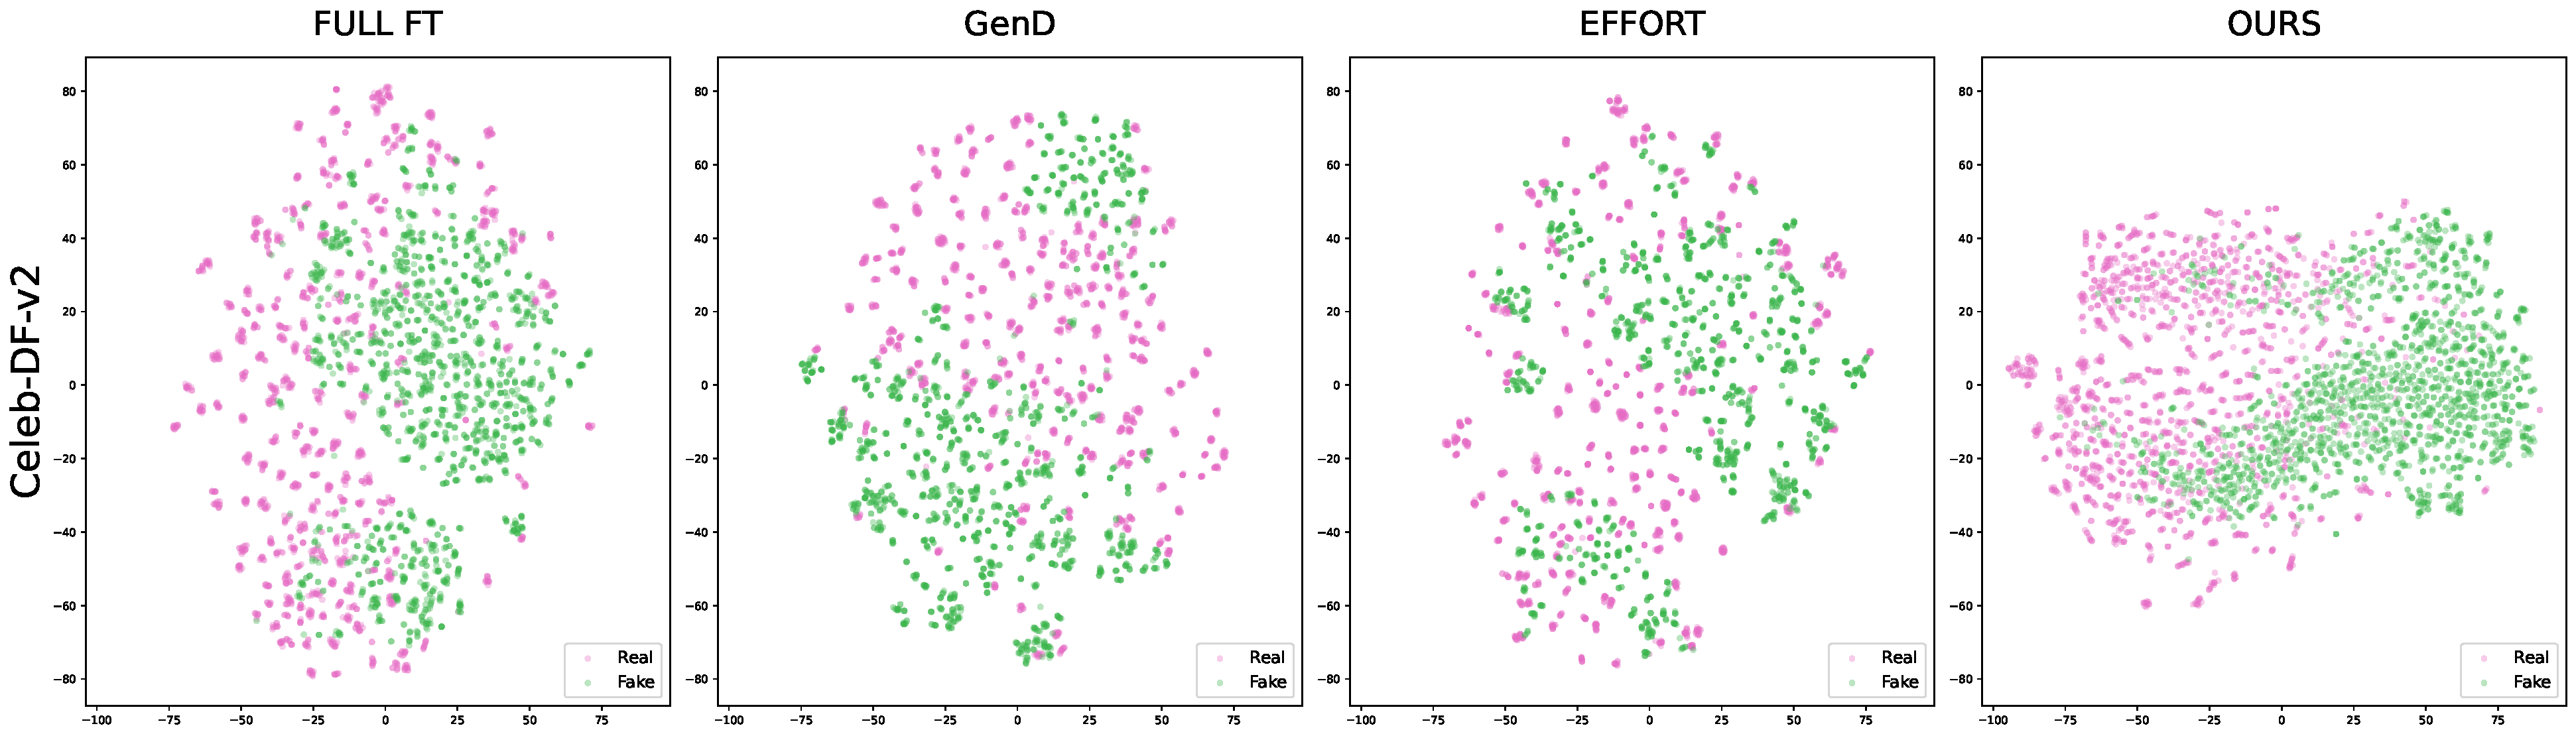
\includegraphics[width=\textwidth]{compare_4models_celebdf_b16_redraw_2.pdf}
    \caption{T-SNE visualization of real and fake feature embeddings from Celeb-DF-v2 for Full FT, GenD, Effort, and BiasLN.}
    \label{fig:celebdf-feature-comparison}
\end{figure*}

To compare what each model learns, we inspect the features on the Celeb-DF-v2 test set. For each sample, we take the output of the last layer before classification and map it to 2D with t-SNE. As shown in Figure~\ref{fig:celebdf-feature-comparison}, BiasLN shows improved separation between real and fake samples than Full FT, GenD~\cite{yermakov2025gend}, and Effort~\cite{yan2025effort}. Although some overlap remains for all methods, BiasLN forms more coherent and discriminative clusters, suggesting stronger representation quality and better cross-domain robustness on Celeb-DF-v2.



\subsection{Importance of Cross-Domain Validation}

\begin{figure}[h]
    \centering
    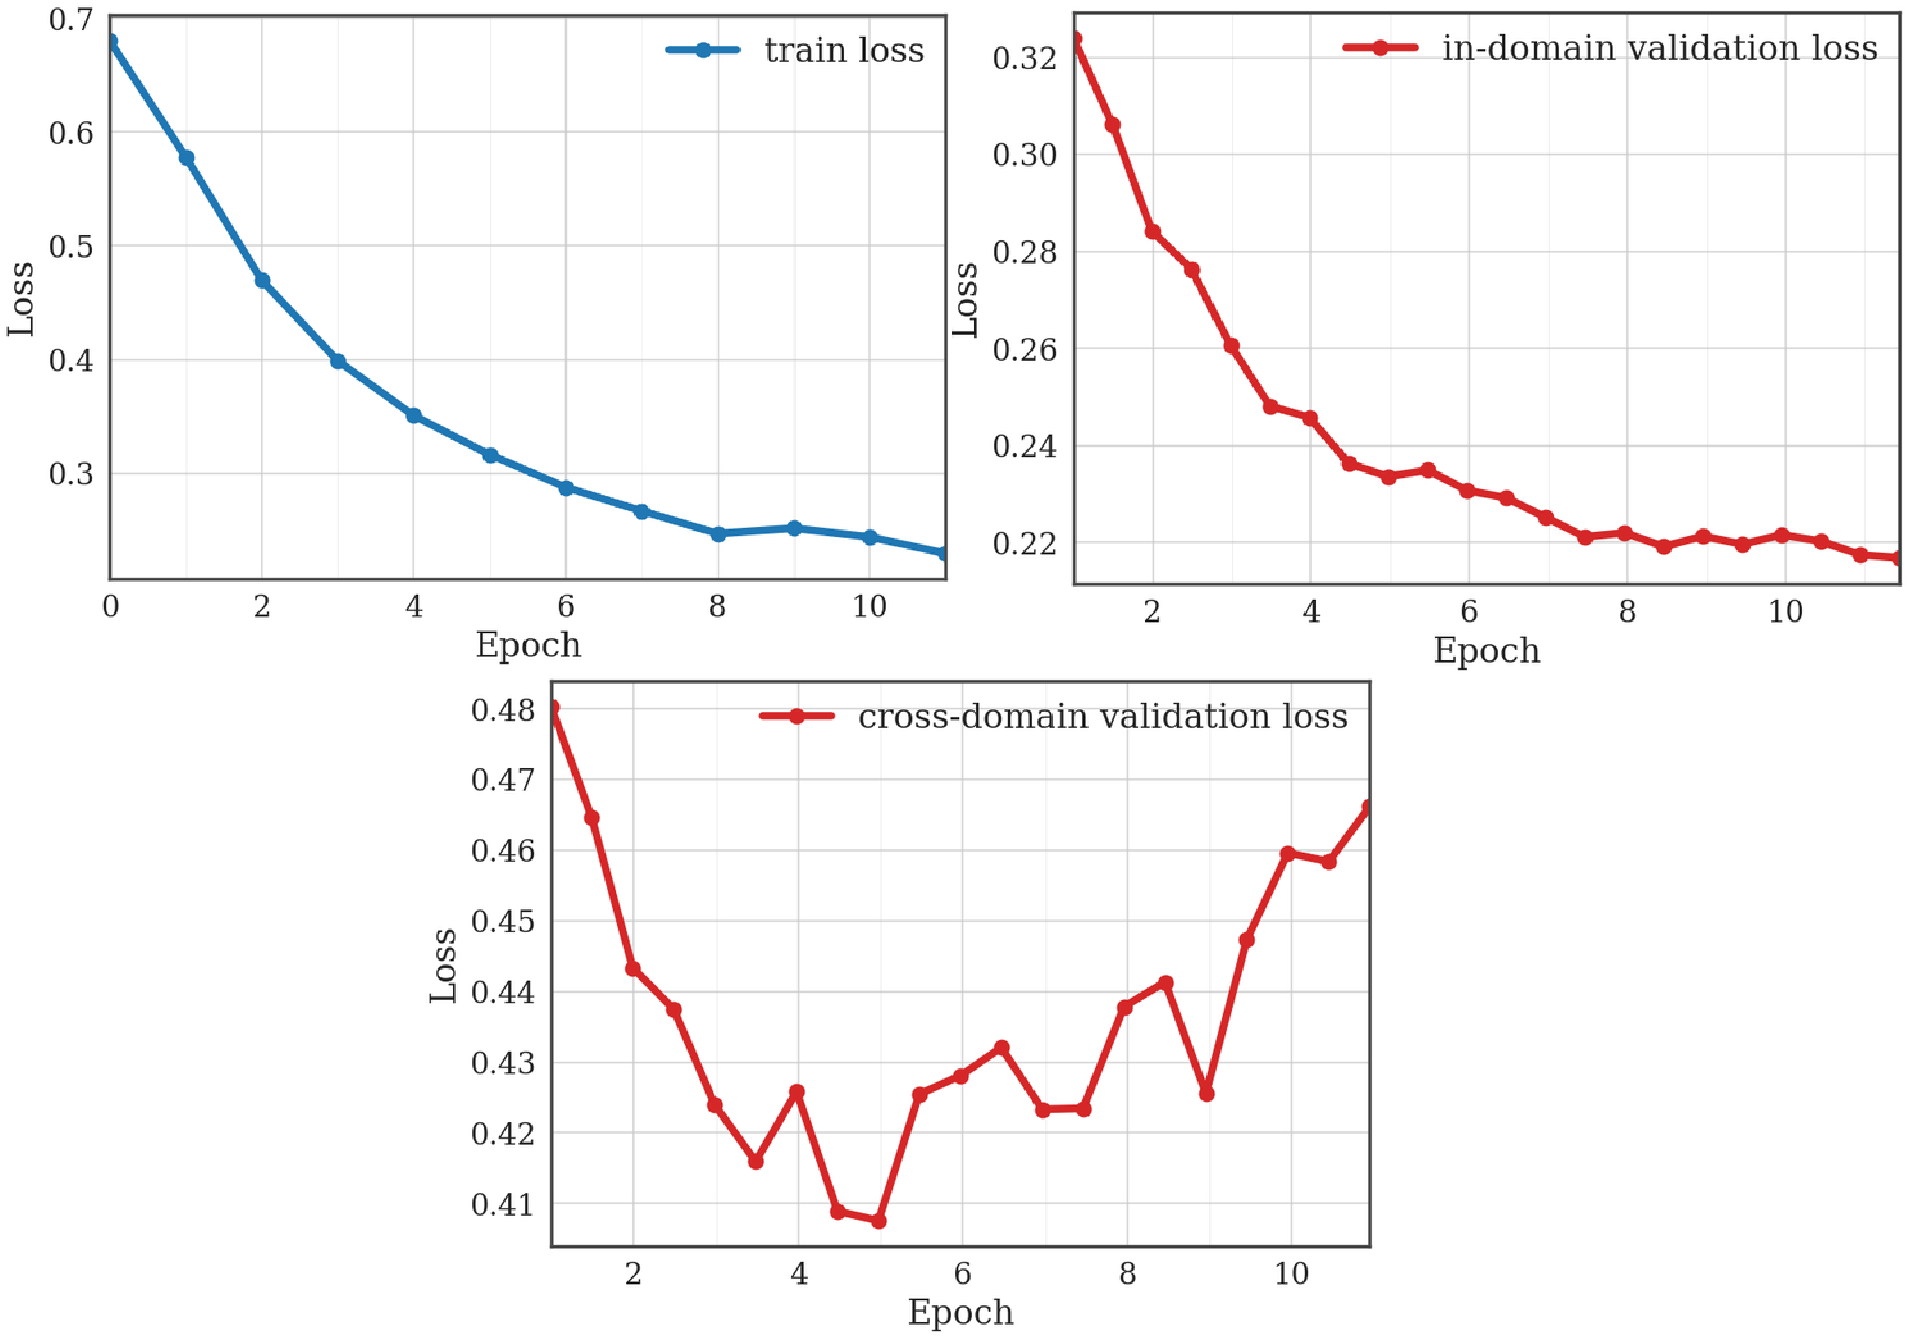
\includegraphics[width=\linewidth]{TrainTestLoss.pdf}
    \captionsetup{justification=centering}
    \caption{Smoothed training and cross-domain validation loss curves of BiasLN.}
    \label{fig:train-test-loss}
\end{figure}    
Figure~\ref{fig:train-test-loss} plots the training loss on the in-domain FF++ dataset alongside the validation loss on a held-out cross-domain subset of Celeb-DF-v2.
These curves reveal an important pattern: when generalization is the objective, validating on the source domain is largely uninformative. Although the in-domain training loss continues to decrease over time, this does not translate into better transfer to unseen datasets. Instead, prolonged training increases the risk of overfitting to source-specific artifacts, and in-domain validation cannot reliably capture this behavior.
As shown in Figure~\ref{fig:train-test-loss}, training for too many epochs degrades generalization to unseen data even when the source-domain loss continues to improve.




\subsection{Ablation Study}
We conduct an ablation study to isolate the effects of parameter-efficient fine-tuning and feature normalization, as summarized in Table~\ref{tab:ablation}.
We begin with a full fine-tuning baseline using a linear classification head and cross-entropy loss, and then replace full fine-tuning with PEFT variants including LoRA, BitFit, LayerNorm tuning, and their combination.
For the PEFT baselines, we additionally compare settings with and without $L_2$ normalization before the linear classifier to examine whether normalized features improve generalization.
All configurations are evaluated under the same protocol, and the results reported in Table~\ref{tab:ablation} are video-level AUC averaged over five runs with different random seeds.

\begin{table}[h]
  \centering
  \captionsetup{labelsep=period, labelfont=bf, hypcap=false}
  \caption{Ablation study of PEFT variants and the effect of $L_2$ normalization before the linear classifier.
Results are reported as video-level AUC averaged over five runs.}
  \label{tab:ablation}
  \footnotesize
  \setlength{\tabcolsep}{3pt}
  \renewcommand{\arraystretch}{1.1}
  \resizebox{\columnwidth}{!}{%
  \begin{tabular}{l c c c cccc c}
    \toprule
    \multirow{2}{*}{\textbf{PEFT Method}} & \multirow{2}{*}{\textbf{Head}} & \multirow{2}{*}{\textbf{$L_2$ Norm}} & \multirow{2}{*}{\textbf{Loss}} & \multicolumn{4}{c}{\textbf{Cross-dataset}} & \multirow{2}{*}{\textbf{Avg}} \\
    \cmidrule(lr){5-8}
    & & & & \textbf{CDF-v2} & \textbf{DFDC} & \textbf{DFD} & \textbf{UADFV} & \\
    \midrule
    Full FT & Linear & No & CE & 0.655 & 0.560 & 0.495 & 0.624 & 0.5835 \\
    LoRA & Linear & No & CE & 0.941 & 0.844 & \textbf{0.977} & 0.988 & 0.9375 \\
    LoRA & Linear & Yes & CE & 0.893 & 0.819 & 0.955 & 0.986 & 0.9133 \\
    BitFit & Linear & No & CE & \cellcolor{gray!15}0.953 & \cellcolor{gray!15}0.846 & 0.969 & \cellcolor{gray!15}0.996 & 0.9410 \\
    BitFit & Linear & Yes & CE & 0.927 & 0.826 & 0.961 & 0.994 & 0.9270 \\
    LayerNorm (LN) & Linear & No & CE & 0.931 & 0.840 & 0.966 & 0.993 & 0.9325 \\
    LayerNorm (LN) & Linear & Yes & CE & 0.945 & \textbf{0.866} & \cellcolor{gray!15}0.973 & \textbf{0.998} & \cellcolor{gray!15}0.9455 \\
    \midrule
    BitFit + LN & Linear & Yes & CE & \textbf{0.971} & \textbf{0.866} & \textbf{0.977} & 0.992 & \textbf{0.9515} \\
    \bottomrule
  \end{tabular}%
  }
\end{table}

\section{Conclusion}

In this paper, we presented BiasLN, a generalized deepfake detection framework that follows the core intuition of Effort~\cite{yan2025effort}: a robust detector should preserve the pre-trained representation space and rely more on the intrinsic structure of real images than on unstable local forgery artifacts.
Instead of tuning the entire backbone, we update only the bias terms and LayerNorm parameters. This helps the model keep more generalizable information without requiring much adaptation.

The results show that this lightweight tuning strategy still works well across different datasets and manipulation methods.
They also reveal an important practical challenge for generalization: checkpoint selection based on a validation split drawn from the source dataset is largely uninformative, because strong source-domain validation performance does not reliably translate to out-of-domain robustness.
In practice, this makes it difficult to identify truly generalizable model weights without a stronger validation protocol.
These findings highlight the importance of preserving pre-trained representations while keeping the adaptation simple, and they support the practical value of parameter-efficient designs for robust deepfake detection.


\section{Limitations and Future Work}
Although our method outperforms current state-of-the-art methods on the benchmark, it still has several limitations that should be addressed in future work.

First, because of limited computing resources, we select the model checkpoint using only a single validation subset during training.
This means that the selected model may not represent the best balance between in-domain performance and cross-domain generalization.
In this study, we use a subset of Celeb-DF-v2 as the validation set, but a more robust future direction would be to construct a validation mixture that combines samples from multiple datasets.
Such a mixed validation set could provide a broader proxy for distribution shift and support more reliable checkpoint selection.

Second, our model works on cropped video frames instead of full video sequences.
Because of this, the model may miss temporal inconsistencies and motion artifacts that only appear across consecutive frames.

Third, strong results on public benchmarks do not eliminate the risk of misuse. As deepfake detectors become more effective, malicious users may use their feedback to create more realistic fake content.

In future work, we will study better validation strategies, such as building a mixed validation set from multiple datasets. We also plan to incorporate temporal modeling for video-level artifacts, evaluate the method on newer manipulation techniques, and examine how it can be deployed more safely in practice.



\begin{thebibliography}{99}
\balance

\bibitem{goodfellow2020gan}
Goodfellow I, Pouget-Abadie J, Mirza M, Xu B, Warde-Farley D, Ozair S, Courville A, Bengio Y.
Generative adversarial networks.
Commun ACM. 2020;63(11):139–44.

\bibitem{yang2022diffusion}
Yang L, Zhang Z, Song Y, Hong S, Xu R, Zhao Y, Zhang W, Cui B, Yang MH.
Diffusion models: A comprehensive survey of methods and applications.
ACM Comput Surv. 2024;62(1). doi:10.1145/3626235. arXiv:2209.00796.

\bibitem{bray2023testing}
Bray SD, Johnson SD, Kleinberg B.
Testing human ability to detect deepfake images of human faces.
J Cybersecur. 2023;9(1):tyad011.

\bibitem{hashmi2024unmasking}
Hashmi A, Shahzad SA, Lin CW, Tsao Y, Wang HM.
Unmasking illusions: Understanding human perception of audiovisual deepfakes.
arXiv Preprint. 2024;arXiv:2405.04097.

\bibitem{yan2025effort}
Yan Z, Wang J, Jin P, Zhang KY, Liu C, Chen S, et al.
Orthogonal subspace decomposition for generalizable AI-generated image detection.
In: Proc Int Conf Mach Learn (ICML). 2025.

\bibitem{benzaken2022bitfit}
Zaken EB, Goldberg Y, Ravfogel S.
BitFit: Simple parameter-efficient fine-tuning for transformer-based masked language models.
In: Proc 60th Annu Meeting Assoc Comput Linguistics (ACL). 2022;2:1–9.

\bibitem{yermakov2025gend}
Yermakov A, Cech J, Matas J, Fritz M.
Deepfake detection that generalizes across benchmarks.
arXiv Preprint. 2025;arXiv:2508.06248.

\bibitem{wang2022ln}
Wang Q, Ruan YP, Zuo Y, Li T.
Parameter-efficient tuning on layer normalization for pretrained language models.
arXiv Preprint. 2022;arXiv:2211.08682.

\bibitem{ojha2023universal}
Ojha U, Li Y, Lee YJ.
Towards universal fake image detectors that generalize across generative models.
In: Proc IEEE/CVF Conf Comput Vis Pattern Recognit (CVPR). 2023;24480–9.

\bibitem{yan2023deepfakebench}
Yan Z, Zhang Y, Yuan X, Lyu S, Wu B.
DeepfakeBench: A comprehensive benchmark of deepfake detection.
Adv Neural Inf Process Syst. 2023;36:4534–65.

\bibitem{yan2024df40}
Yan Z, Zhang Y, Yuan X, Lyu S, Wu B.
DF40: Toward next-generation generalizable deepfake detection.
In: Proc IEEE/CVF Conf Comput Vis Pattern Recognit Workshops (CVPRW). 2024.


\bibitem{yan2023ucf}
Yan Z, Zhang Y, Fan Y, Wu B.
UCF: Uncovering common features for generalizable deepfake detection.
In: Proc IEEE/CVF Int Conf Comput Vis (ICCV). 2023.

\bibitem{yan2024latent}
Yan Z, Luo Y, Lyu S, Liu Q, Wu B.
Transcending forgery specificity with latent space augmentation for generalizable deepfake detection.
In: Proc IEEE/CVF Conf Comput Vis Pattern Recognit (CVPR). 2024.

\bibitem{rossler2019ff}
Rossler A, Cozzolino D, Verdoliva L, Riess C, Thies J, Niessner M.
FaceForensics++: Learning to detect manipulated facial images.
In: Proc IEEE/CVF Int Conf Comput Vis (ICCV). 2019.

\bibitem{qian2020frequency}
Qian Y, Yin G, Sheng L, Chen Z, Shao J.
Thinking in frequency: Face forgery detection by mining frequency-aware clues.
In: Proc Eur Conf Comput Vis (ECCV). 2020.

\bibitem{kumar2022finetuning}
Kumar A, Raghunathan A, Jones R, Ma T, Liang P.
Fine-tuning can distort pretrained features and underperform out-of-distribution.
In: Int Conf Learn Representations (ICLR). 2022.

\bibitem{dosovitskiy2021vit}
Dosovitskiy A, Beyer L, Kolesnikov A, Weissenborn D, Zhai X, Unterthiner T, et al.
An image is worth 16x16 words: Transformers for image recognition at scale.
In: Int Conf Learn Representations (ICLR). 2021.

\bibitem{hu2022lora}
Hu EJ, Shen Y, Wallis P, Allen-Zhu Z, Li Y, Wang S, et al.
LoRA: Low-rank adaptation of large language models.
In: Int Conf Learn Representations (ICLR). 2022.

\bibitem{wang2020alignment}
Wang T, Isola P.
Understanding contrastive representation learning through alignment and uniformity on the hypersphere.
In: Proc Int Conf Mach Learn (ICML). 2020.

\bibitem{radford2021clip_vitl}
Radford A, Kim J, Hallacy C, Ramesh A, Goh G, Agarwal S, et al.
Learning transferable visual models from natural language supervision.
In: Int Conf Mach Learn (ICML). 2021;8748–63.


\bibitem{caron2021emerging}
Caron M, Touvron H, Misra I, J{\'e}gou H, Mairal J, Bojanowski P, Joulin A.
Emerging properties in self-supervised vision transformers.
In: Proc IEEE/CVF Int Conf Comput Vis (ICCV). 2021.

\bibitem{giannou2023layernorm}
Giannou A, Rajput S, Papailiopoulos D.
The expressive power of tuning only the normalization layers.
arXiv Preprint. 2023;arXiv:2302.07937.

\bibitem{valizadeh2024layernorm}
ValizadehAslani T, Liang H.
LayerNorm: A key component in parameter-efficient fine-tuning.
arXiv Preprint. 2024;arXiv:2403.20284.

\bibitem{deng2020retinaface}
Deng J, Guo J, Ververas E, Kotsia I, Zafeiriou S.
RetinaFace: Single-shot multi-level face localisation in the wild.
In: Proc IEEE/CVF Conf Comput Vis Pattern Recognit (CVPR). 2020.

\bibitem{sagonas2016}
Sagonas C, Antonakos E, Tzimiropoulos G, Zafeiriou S, Pantic M.
300 Faces in-the-Wild Challenge: Database and results.
Image Vis Comput. 2016;47:3–18.

\bibitem{liu2021spsl}
Liu H, Li X, Zhou W, Chen Y, He Q, Xiong H, et al.
Spatial-phase shallow learning: Rethinking face forgery detection in frequency domain.
In: Proc IEEE/CVF Conf Comput Vis Pattern Recognit (CVPR). 2021.

\bibitem{luo2021srm}
Luo H, Zhang B, Liu S, Li H, Chen H, Wen B, et al.
Generalizing face forgery detection with high-frequency features.
In: Proc IEEE/CVF Conf Comput Vis Pattern Recognit (CVPR). 2021.

\bibitem{ni2022core}
Ni Y, Meng Y, Yu C, Qu J, Chen J, Jiang Y.
CORE: Consistent representation learning for face forgery detection.
In: Proc IEEE/CVF Conf Comput Vis Pattern Recognit Workshops (CVPRW). 2022.

\bibitem{cao2022recce}
Cao J, Ma C, Yao T, Chen S, Ding T, Yang X.
End-to-end reconstruction-classification learning for face forgery detection.
In: Proc IEEE/CVF Conf Comput Vis Pattern Recognit (CVPR). 2022.

\bibitem{gu2022slad}
Gu Z, Chen W, Bao S, Ding W, Zhang B, Chen H, et al.
Leveraging real talking faces via self-supervised audio-visual speech representation learning for deepfake video detection.
In: Proc IEEE/CVF Conf Comput Vis Pattern Recognit (CVPR). 2022.

\bibitem{shiohara2022sbi}
Shiohara K, Yamasaki T.
Detecting deepfakes with self-blended images.
In: Proc IEEE/CVF Conf Comput Vis Pattern Recognit (CVPR). 2022.

\bibitem{huang2023iid}
Huang M, Bhunia B, Bhatt P.
IID: Instance-inconsistency detection for generalizable deepfake detection.
In: Proc IEEE/CVF Conf Comput Vis Pattern Recognit (CVPR). 2023.

\bibitem{sun2024lsda}
Sun K, Liu Z, Tan H, Chen C.
LSDA: Large scale deepfake detection augmentation.
In: Proc IEEE/CVF Conf Comput Vis Pattern Recognit (CVPR). 2024.

\bibitem{yang2024prodet}
Yang Z, Xu J, Zhao B, Wang M.
ProDet: Progressive detection for generalizable deepfake detection.
In: Proc AAAI Conf Artif Intell. 2024.

\bibitem{lin2024cdfa}
Lin X, Liu Z, Ouyang W.
CDFA: Cross-domain feature alignment for generalizable deepfake detection.
In: Proc IEEE/CVF Conf Comput Vis Pattern Recognit (CVPR). 2024.

\bibitem{cui2025forada}
Cui Z, Zhang Y, Yao T, Ding S, Wu B, Yuan L.
ForAda: Forgery-aware adaptive transformer for generalizable deepfake detection.
In: Proc IEEE/CVF Conf Comput Vis Pattern Recognit (CVPR). 2025.

\bibitem{badr2025wavit}
Badr NEA, Nebel JC, Greenhill D, Liang X.
WaViT-CDC: Wavelet vision transformer with central difference convolutions for spatial-frequency deepfake detection.
IEEE Open J Signal Process. 2025;6:621–30. doi:10.1109/OJSP.2025.3571679.

\bibitem{li2018ictu}
Li Y, Chang MC, Lyu S.
In Ictu Oculi: Exposing AI created fake videos by detecting eye blinking.
In: Proc IEEE Int Workshop Inf Forensics Secur (WIFS). 2018.

\bibitem{li2020celeb}
Li Y, Yang X, Sun P, Qi H, Lyu S.
Celeb-DF: A large-scale challenging dataset for deepfake forensics.
In: Proc IEEE/CVF Conf Comput Vis Pattern Recognit (CVPR). 2020;3207–16.

\bibitem{dufour2019dfd}
Dufour N, Gully A.
Contributing data to deepfake detection research.
Google AI Blog. 2019. Available from: https://googleblog.com.

\bibitem{dolhansky2019dfdcp}
Dolhansky B, Howes R, Pflaum B, Baram N, Ferrer CC.
The deepfake detection challenge (DFDC) preview dataset.
arXiv Preprint. 2019;arXiv:1910.08854.

\bibitem{dolhansky2020dfdc}
Dolhansky B, Bitton J, Pflaum B, Lu J, Howes R, Wang M, et al.
The deepfake detection challenge (DFDC) dataset.
arXiv Preprint. 2020;arXiv:2006.07397.

\end{thebibliography}
\cleardoublepage
\begin{figure*}[b]
    \centering
    \captionsetup{justification=centering}
    \adjustbox{max totalsize={\textwidth}{0.9\textheight},center}{
        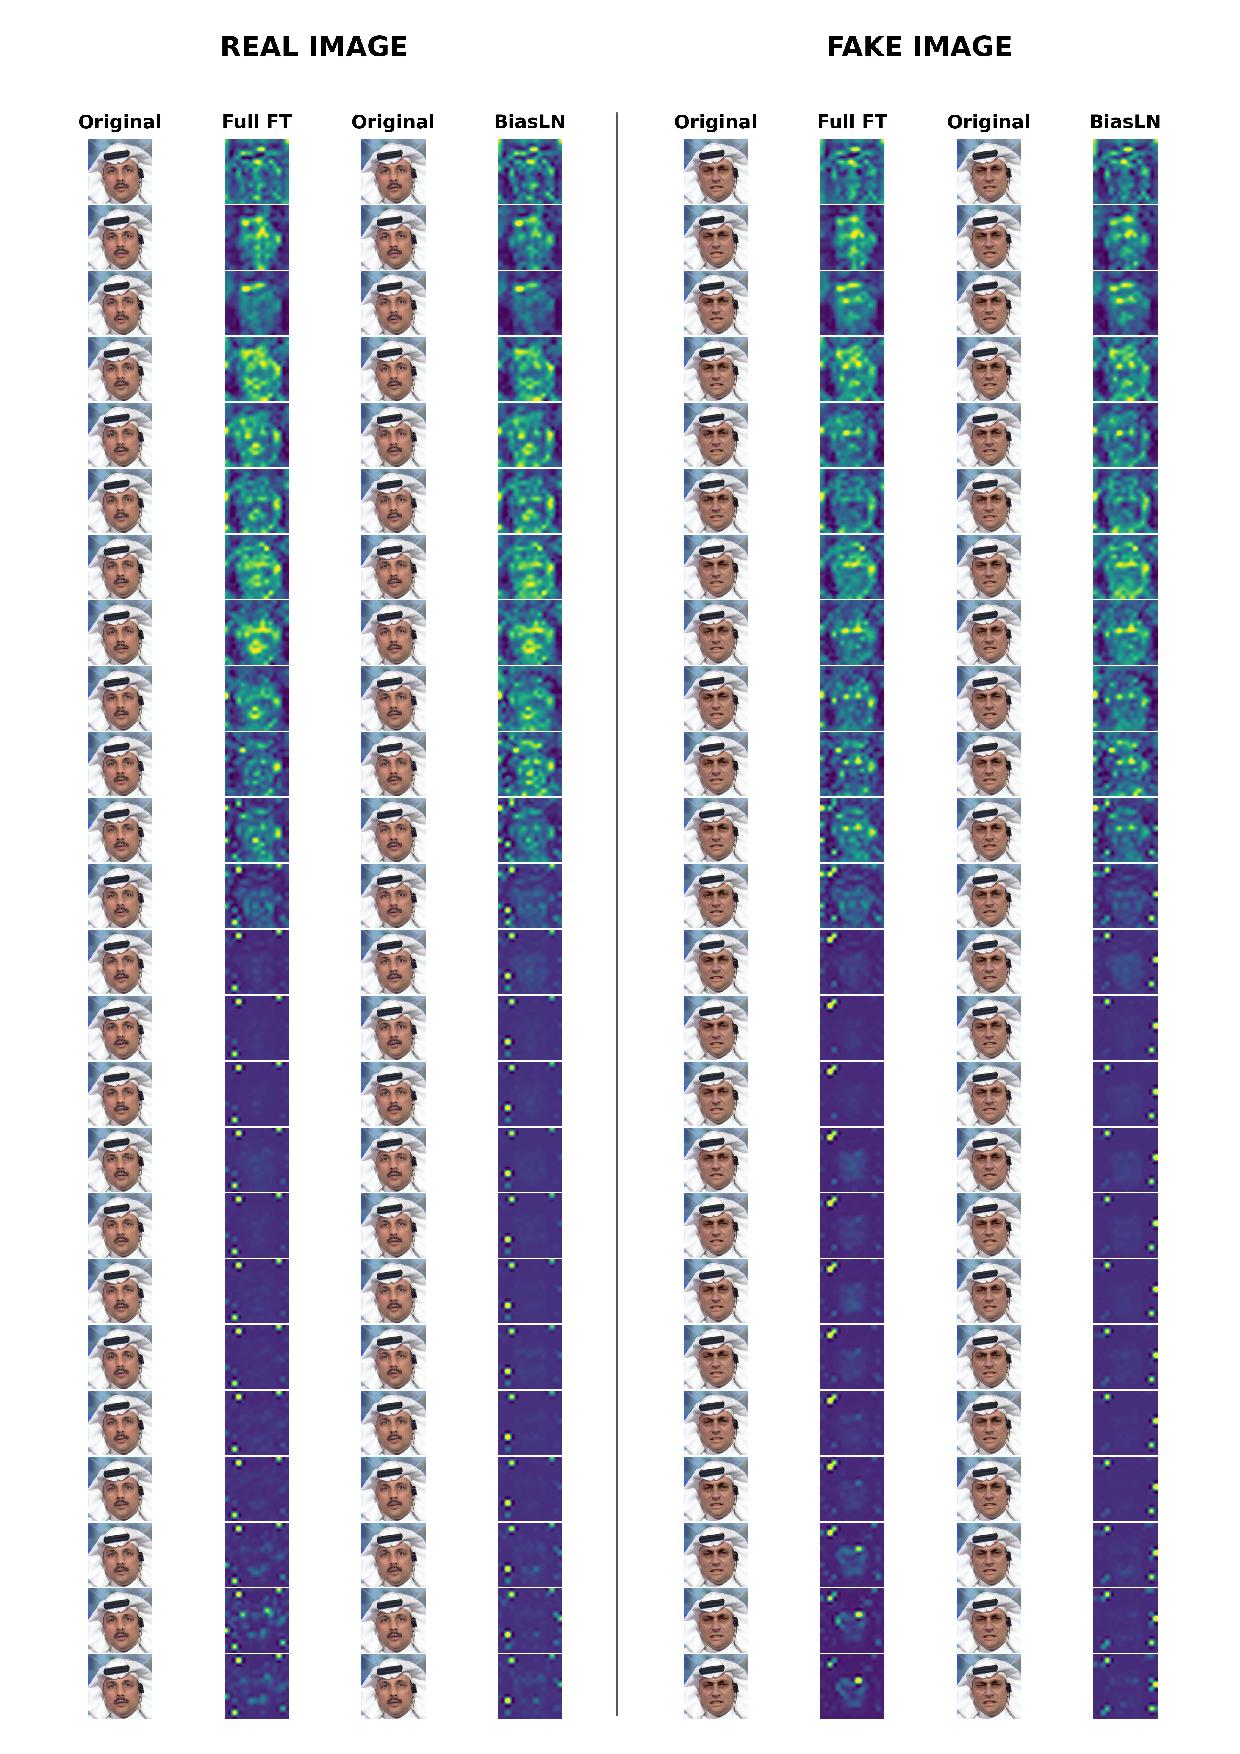
\includegraphics[width=\textwidth]{self_attention_map.pdf}
    }
    \caption{Visualization of self-attention maps for a fake image from FF++ and its corresponding real image across all blocks of the CLIP-ViT model. The model contains 24 blocks, whose IDs increase from top to bottom.}
    \label{fig:self-attention-map}
\end{figure*}



\end{document}